\section{Concept Map}

Das Thema der vorliegenden Arbeite ist die Ausarbeitung des Algorithmus der Breitensuche in Form Lernprogrammartiger Unterlagen für das Gymnasium.  
Zu diesem Zweck wurde folgende Concept-Map entworfen, die sowohl das Vorwissen als auch einen kleinen Ausblick auf weitere Themen geben soll.
Dabei wurde Konzept, welches als Vorwissen schon bekannt sein sollte, aber im Rahmen dieser Arbeit nochmal wiederholt werden soll, blau gefärbt. 
Neue Konzepte, die in dieser Arbeit behandelt und eingeführt werden sollen, wurden grün gefärbt. 
Weitere Konzepte, die nicht mehr in dieser Arbeit behandelt werden, wurden orange gefärbt. 

\begin{figure}[htb]
\begin{center}
%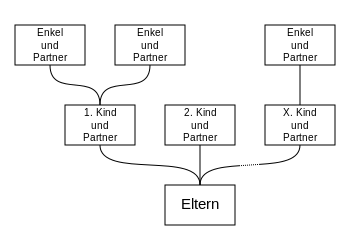
\includegraphics[width=.7\textwidth]{../fig/stammbaum.png}
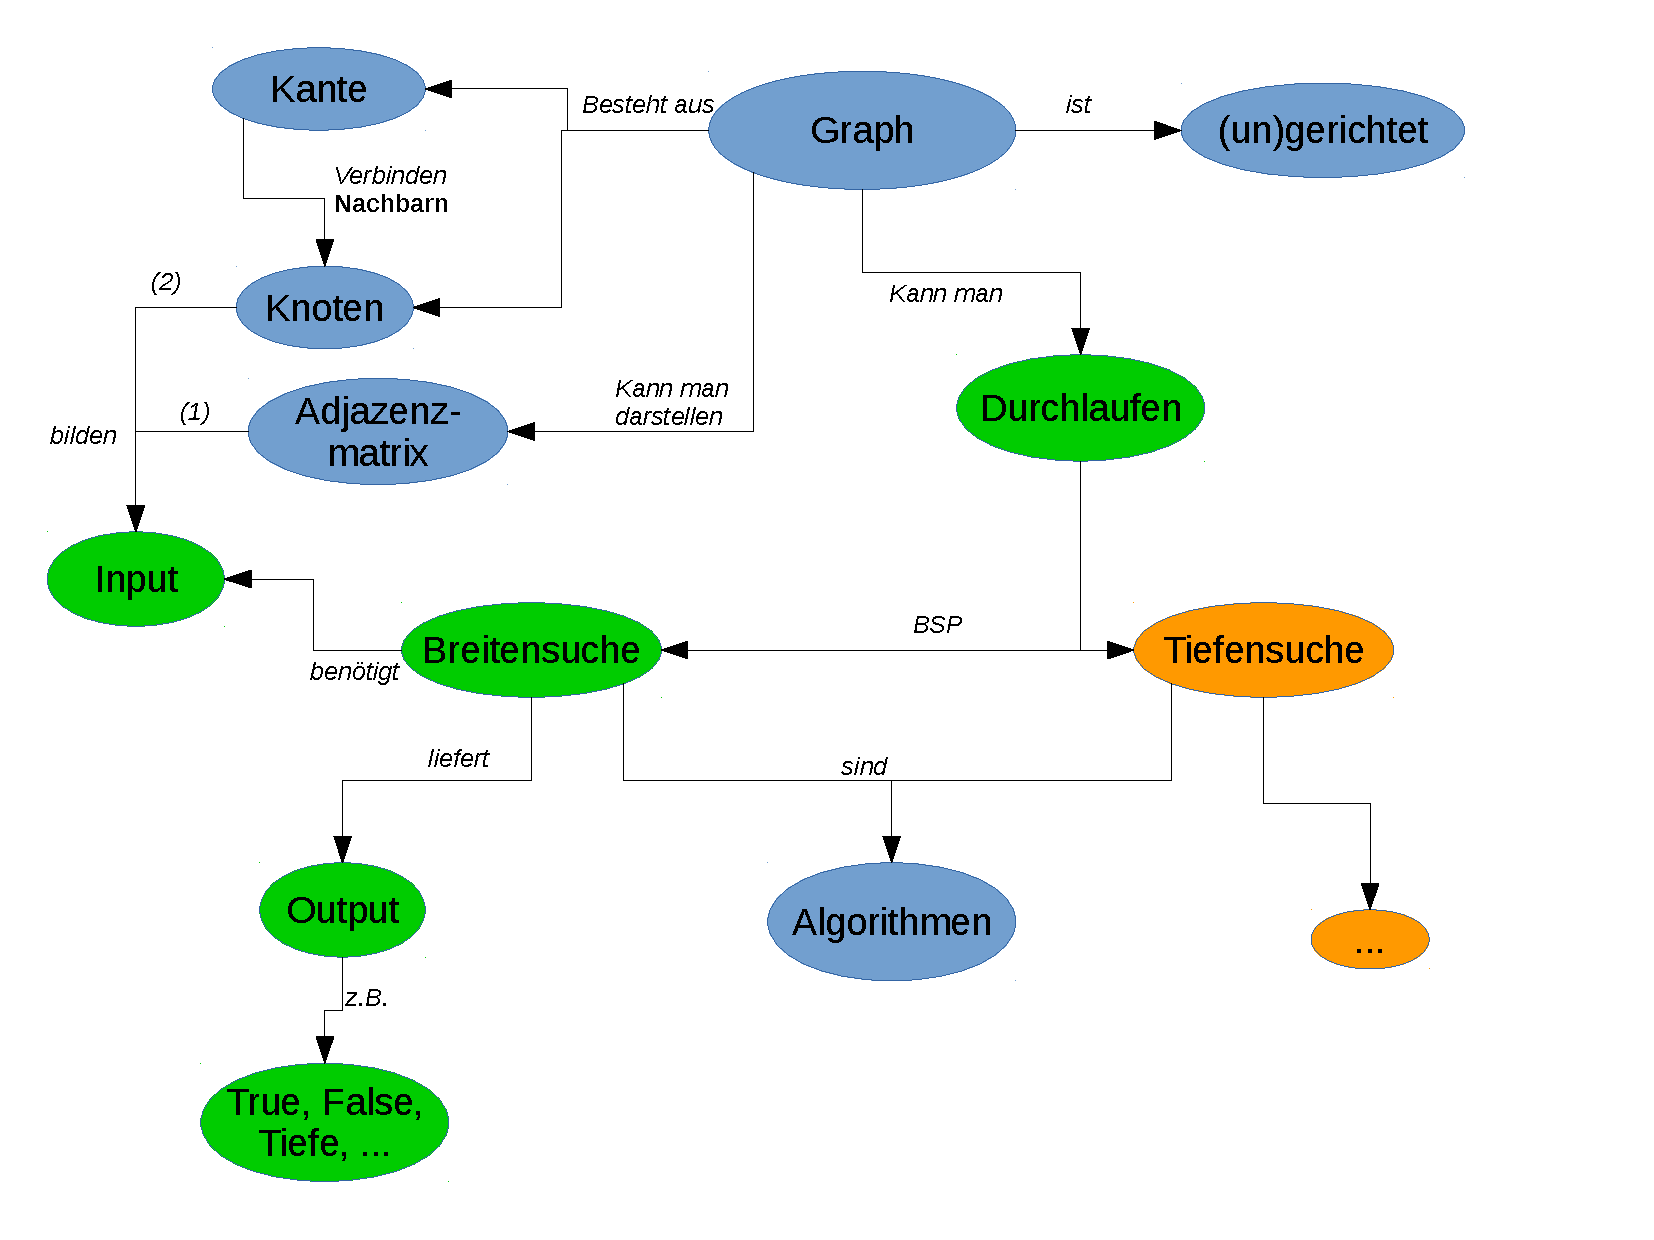
\includegraphics[width=.99\textwidth]{../cmap/bsuche_cmap.pdf}
\caption{Concept-Map zum Thema Breitensuche.
Blaue Konzepte bilden das Vorwissen ab. Grüne Konzepte werden in dieser Arbeit eingeführt und behandelt. Orange Konzepte bilden einen Ausblick auf Konzepte, welche im Rahmen dieser Arbeit nicht mehr behandelt werden können. 
}
\label{fig:cmap}
\end{center}
\end{figure}


\section{Lernziele}

Aus dieser Concept-Map lassen sich folgende Lernziele für diese Arbeit ableiten. 

\subsection{Leitidee}

Graphen spielen eine wichtige Rolle in unserem Alltag (S-Bahnnetzwerk, Facebook, Websites, \dots). 
Mit diesen Netzwerken sind viele Fragen verbunden: Über wie viel Freundschaften bin ich mit einer anderen Person verbunden? Wie lange ist die kürzeste Verbindung von A nach B?
Damit man ein grundlegendes Verständnis dafür entwickelt, muss man sich überlegen, wie man sich auf Graphen bewegen kann. 
Eine Möglichkeit bietet die Breitensuche, welche einen naiven Einstieg bildet. 


\subsection{Dispositionsziel}

Die SuS wissen, dass man mit gewisse Probleme mit Hilfe von Graphen modellieren und mit Graphenalgorithmen lösen kann. 
Sie können Probleme analysieren und beurteilen, ob sie mit Hilfe von einer Breitensuche in einem Graphen gelöst werden können.



\subsection{Operationalisierte Lernziele}

\begin{enumerate}
\item Die SuS kennen die Begriffe zur Darstellung von einfachen Graphen: (un)gerichtet, Knoten und Kante.

\item Die SuS kennen verschiedene Darstellungsmöglichkeiten von Graphen und können diese ineinander überführen: Zeichnung, Knoten- /Kantenmenge und Adjazenzmatrix.

\item Die SuS können die Nachbarn von Knoten auf verschieden Darstellungen von Graphen bestimmen. 

\item Die SuS können ein Programm schreiben, welches die Nachbarn eines Knoten eines bestimmten Knoten eines beliebigen Graphen ausgibt.
\end{enumerate}


\dots
Operationalisierte Lernziele:
Die SuS können die Funktionsweise einer Breitensuche in einem Graphen beschreiben
Die SuS können für ein gegebenes Problem Breitensuche in einem Graphen anwenden
Die SuS können ein gegebenes Problem mit einem Graphen modellieren und mittels Breitensuche eine Lösung finden (evtl. spezifischer)
Die SuS können die Breitensuche in TigerJython implementieren
Die SuS können die Laufzeit einer Breitensuche beurteilen (sofern O notation bekannt…)
Die SuS können den Speicherbedarf der Breitensuche beurteilen